We compare the Qwen3-VL series with other models of comparable size on document-related benchmarks, including OCR, document parsing, document question answering (QA), and document reasoning.

We evaluate our flagship model, \ModelBig, against state-of-the-art VLMs on the benchmarks listed in Table~\ref{tab:results_flagship}. On OCR-focused parsing benchmarks — including CC-OCR~\citep{yang2024ccocrcomprehensivechallengingocr} and OmniDocBench~\citep{ouyang2024omnidocbenchbenchmarkingdiversepdf} — as well as comprehensive OCR benchmarks such as OCRBench~\citep{Liu_2024_OCRBench} and OCRBench\_v2~\citep{fu2024ocrbenchv2improvedbenchmark}, the \InstructBig model establishes a new state of the art, marginally outperforming its “thinking” counterpart, \ThinkBig.
On OCR-related visual question answering (VQA) benchmarks that require both OCR capability and keyword search — such as DocVQA~\citep{docvqa}, InfoVQA~\citep{Mathew2021InfographicVQA}, AI2D~\citep{Kembhavi2016AI2D}, ChartQA~\citep{masry2022chartqa}, and the CharXiv~\citep{wang2024charxiv} description subset — both the Instruct and Thinking variants achieve comparable performance, demonstrating consistently strong results across these tasks.
Notably, on the reasoning subset of CharXiv — which demands deep chart comprehension and multi-step reasoning — the Thinking variant surpasses the Instruct version and ranks second only to GPT5-thinking and Gemini-2.5-Pro-Thinking.

Furthermore, among the smaller-sized variants in the Qwen3-VL series, both Qwen3-VL-30BA3B models and Qwen3-VL-32B models consistently outperform Gemini-2.5-Flash and GPT-5-mini across most evaluation metrics, as shown in~\cref{tab:results_medium}. Even the compact dense models — Qwen3-VL-8B, Qwen3-VL-4B, and Qwen3-VL-2B — demonstrate remarkably competitive performance on OCR parsing, visual question answering (VQA), and comprehensive benchmark suites, as detailed in~\cref{tab:results_small}. This highlights the exceptional efficiency and strong scalability of the Qwen3-VL architecture across model sizes.

In this version of the Qwen3-VL, we have placed particular emphasis on enhancing its ability to understand long documents. As reported in~\cref{tab:results_flagship}, in the comparison within the flagship models on the MMLongBench-Doc benchmark~\citep{ma2024mmlongbench}, our \ModelBig achieves overall accuracy of 57.0\%/56.2\% under the instruct/thinking settings, showcasing the SOTA performance on the long document understanding task.

% Furthermore, to broaden the model's utility, we have significantly improved its multilingual OCR capabilities. We curated a comprehensive test set for 39 languages to assess this enhancement. As detailed in \cref{fig:multi_lan_ocr}, Qwen3-VL achieves usable performance (accuracy > 70\%) on 32 different languages, ranging from high-resource languages like French and German to lower-resource ones like Swahili and Cebuano. This result underscores the model's versatility and its potential for deployment in diverse linguistic environments.

Beyond its strong performance on established benchmarks, we have also made substantial strides in multilingual support. This represents a major expansion from the 10 non-English/Chinese languages supported by Qwen2.5-VL to 39 languages in Qwen3-VL. We assess this expanded capability on a newly constructed, in-house dataset. As illustrated in \cref{fig:multi_lan_ocr}, the model's accuracy surpasses 70\%—a threshold we consider practical for real-world usability—on 32 out of the 39 languages tested. This demonstrates that the strong OCR capabilities of Qwen3-VL are not confined to a handful of languages but extend across a broad and diverse linguistic spectrum.

% \begin{figure}
%     \centering
%     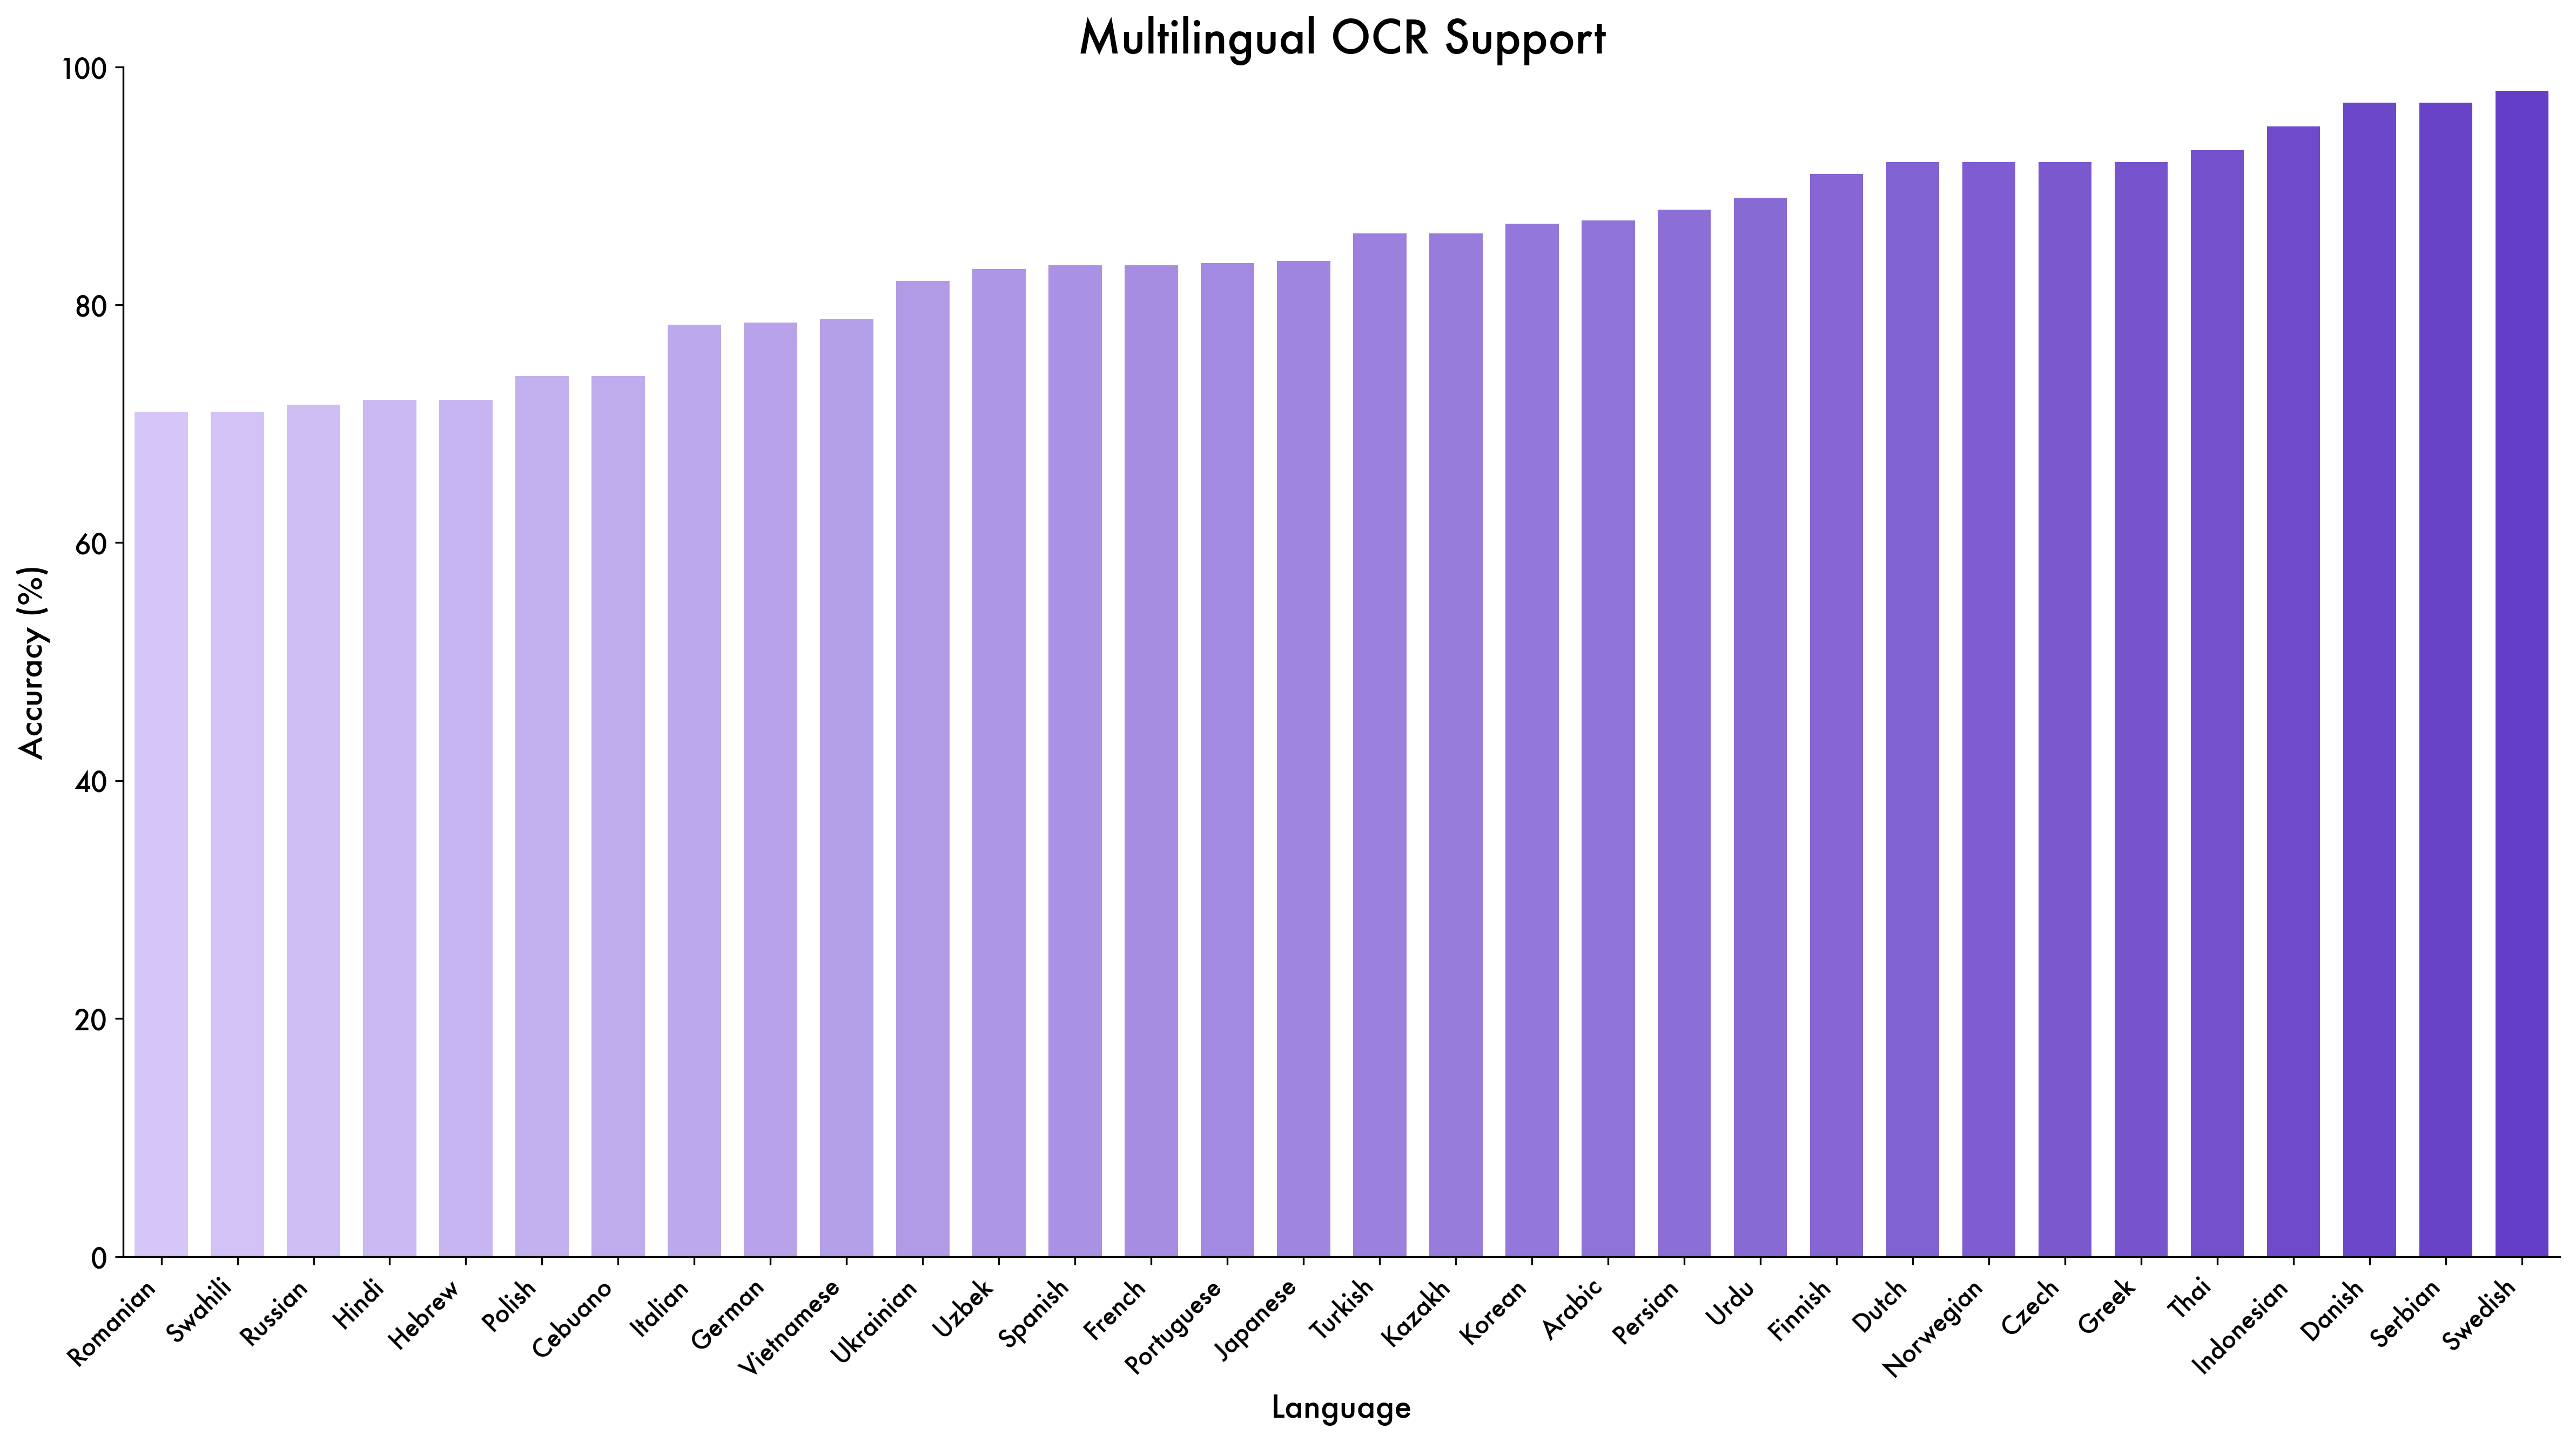
\includegraphics[width=0.9\linewidth]{figures/multi_lan_ocr_support.png}
%     \caption{Multilingual OCR performance of our model on a self-built test set. The model achieves over 70\% accuracy on 32 out of 39 supported languages, demonstrating strong and usable multilingual capabilities.}
%     \label{fig:multi_lan_ocr}
% \end{figure}

\begin{figure}
    \centering
    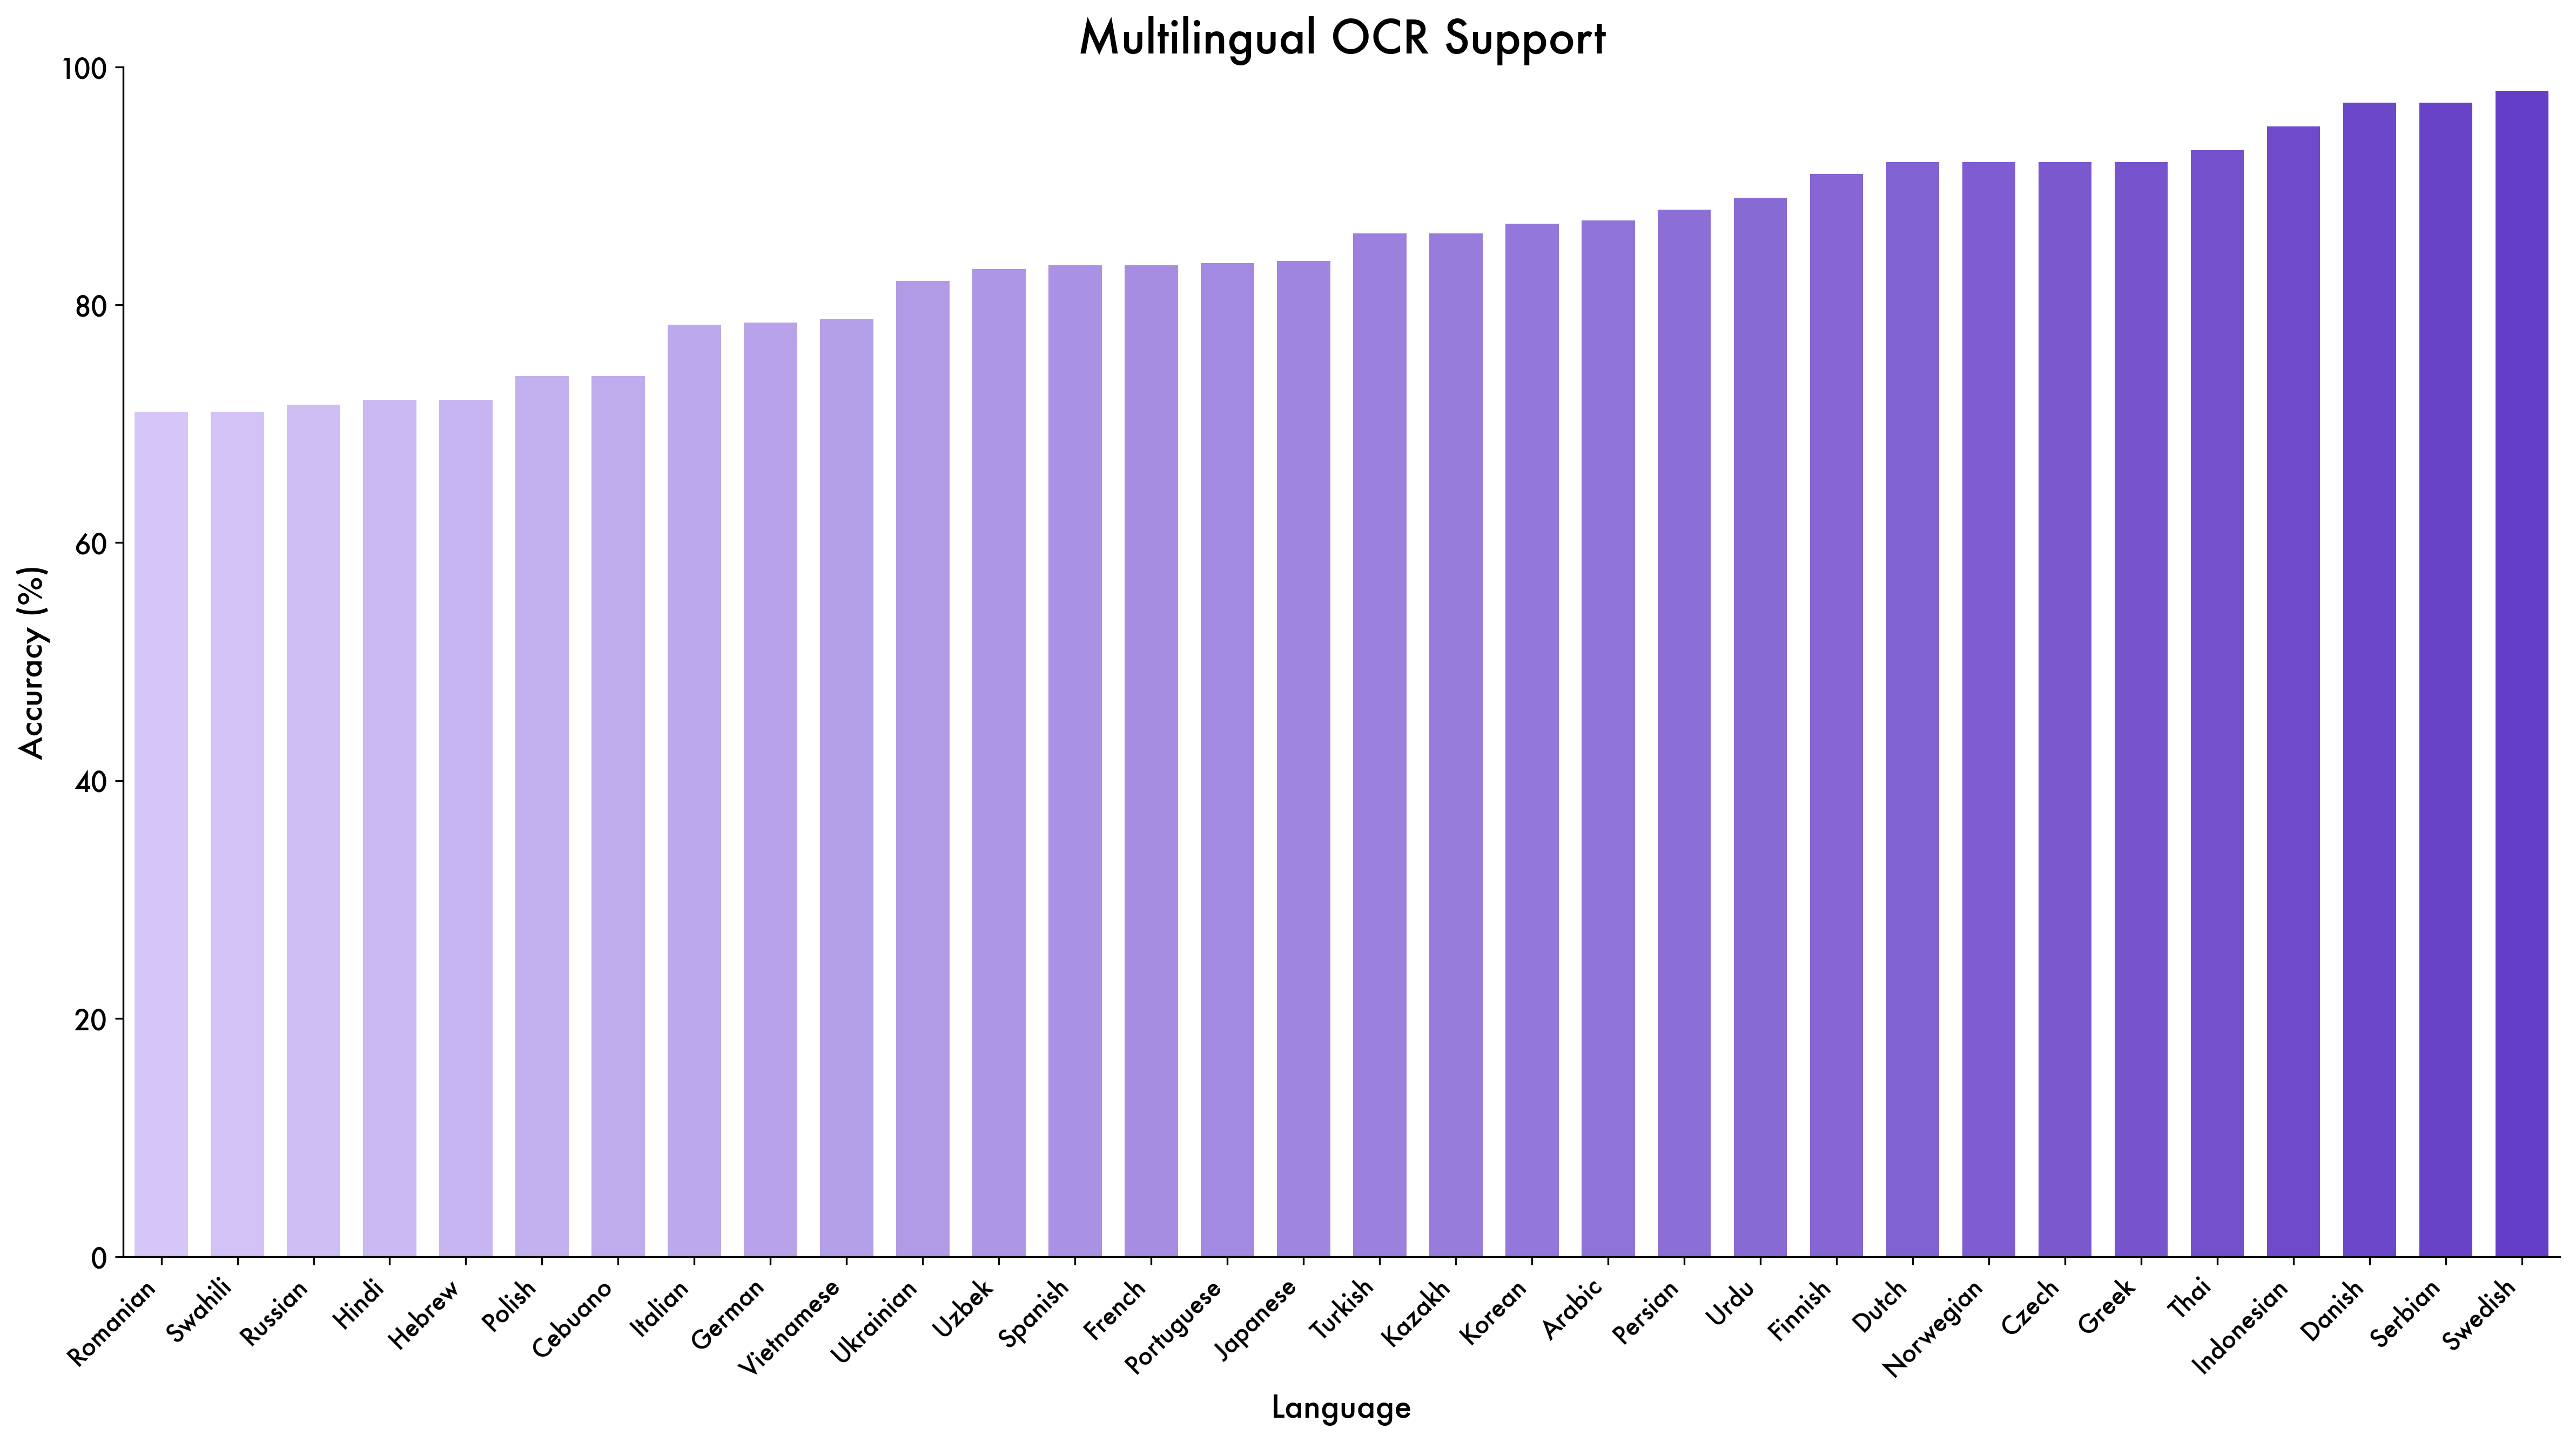
\includegraphics[width=0.85\linewidth]{figures/multi_lan_ocr_support.png}
    \caption{Multilingual OCR performance of our model on a self-built test set. The model achieves over 70\% accuracy on 32 out of 39 supported languages, demonstrating strong and usable multilingual capabilities.}
    \label{fig:multi_lan_ocr}
\end{figure}

%\paragraph{Long Document Understanding.}To measure the model's long document understanding ability, we report the performance of Qwen3-VL and other popular models on MMLongBench-Doc~\citep{ma2024mmlongbench}. For the pre-processing of testing PDF files, we follow previous work~\citep{ma2024mmlongbench} and feed page-sequential PNG-style images into LVLMs. During inference, we use the official recommended parameters for this document scenario. Note that for models such as the Claude series, there is a maximum limit on the number of input images. We concatenate multiple pages to reduce the total number of images.

\begin{comment}
\begin{table}[t]
\centering
\caption{\textbf{Performance of Qwen3-VL-235BA22B and other models on text recognition and document understanding benchmarks.}}
\label{tab:ocr-235a22}
% \small
\setlength{\tabcolsep}{3.0pt}
\scalebox{0.83}{
\begin{tabular}{ccc|cccccc} \toprule
     \multirow[t]{3}{*}{\textbf{Benchmark}} & \textbf{Qwen3-VL} & \textbf{Qwen3-VL} & \textbf{Gemini} & \textbf{Gemini} & \textbf{OpenAI}  & \textbf{OpenAI}  & \textbf{Claude} & \textbf{Claude}  \\
    &  \textbf{235BA22B} & \textbf{235BA22B} & \textbf{2.5 Pro}& \textbf{2.5 Pro} & \textbf{GPT5}  & \textbf{GPT5} & \textbf{opus 4.1} & \textbf{opus 4.1}  \\
    &  {\scriptsize thinking} & {\scriptsize instruct} & {\scriptsize thinking} & {\scriptsize budget-128} & {\scriptsize thinking} & {\scriptsize no-thinking}& {\scriptsize thinking} & {\scriptsize no-thinking}  \\ 
\midrule

DocVQA$_{test}$ & 96.5 & \textbf{97.1} & 92.6 & 94.0 & 91.5 & 89.6 & 92.5 & 89.2 \\  
InfoVQA$_{test}$ & \textbf{89.5} & 89.2 & 84.2 & 82.9 & 79.0 & 69.9 & 69.4 & 60.9 \\
AI2D$_{\text{w. M.}}$ & 89.2 & 89.7 & \textbf{90.9} & 90.0 & 89.7 & 84.1 & 86.4 & 84.4 \\
ChartQA$_{test}$ & \textbf{90.3} & \textbf{90.3} & 83.3 & 62.6 & 59.7 & 59.1 & 86.2 & 83.9 \\
OCRBench & 875 & \textbf{920} & 866 & 872 & 810 & 787 & 764 & 750 \\
OCRBench\_v2$_{\text{en/zh}}$ & 66.8/\textbf{63.5} & \textbf{67.1}/61.8 & 54.3/48.5 & 55.2/53.1 & 53.0/43.2 & 48.2/37.7 & 48.4/43.7 & 47.2/38 \\
CC-OCR & 81.5 & \textbf{82.2} & 77.2 & 76.8 & 68.3 & 66.1 & 69.1 & 66.0 \\
OmniDocBench$_{\text{en/zh}}$$\downarrow$ & 0.201/0.207 & \textbf{0.143}/\textbf{0.207} & 0.347/0.238 & 0.206/0.249 & 0.356/0.472 & 0.174/0.389 & 0.194/0.293 & - \\
CharXiv(DQ) & \textbf{90.5} & 89.4 & 94.4 & 87.8 & 89.2 & 79.5 & 88.5 & 87.8 \\
CharXiv(RQ) & 66.1 & 62.1 & 67.9 & 62.9 & \textbf{81.1} & 57.8 & 63.6 & 60.2 \\
MMLongBench-DOC & 56.2 & 57.0 & 55.6 & 51.2 & 51.5 & 42.4 & 54.5 & 48.1 \\
\bottomrule
\end{tabular}
}
\end{table}


\begin{table}[ht]
\centering
\caption{\textbf{Performance of Qwen3-VL-30BA3B, Qwen3-VL-32B and other models on text recognition and document understanding benchmarks.}}
\label{tab:ocr-30a3}
% \small
\begin{adjustbox}{max width=1\textwidth}
\begin{tabular}{ccc|cc|cccc} \toprule
     \multirow[t]{3}{*}{\textbf{Benchmark}} & \textbf{Qwen3-VL} & \textbf{Qwen3-VL} & \textbf{Qwen3-VL} & \textbf{Qwen3-VL} & \textbf{Gemini2.5}  & \textbf{Gemini2.5}  & \textbf{Qwen2.5-VL}   \\
    &  \textbf{30BA3B} & \textbf{30BA3B} & \textbf{32B}& \textbf{32B} & \textbf{flash}  & \textbf{flash} & \textbf{72B}  \\
    &  {\scriptsize thinking} & {\scriptsize instruct} & {\scriptsize thinking} & {\scriptsize instruct} & {\scriptsize thinking} & {\scriptsize nothinking}& {\scriptsize nothinking}  \\ 
\midrule
DocVQA$_{test}$ & 95.5 & 95.0 & 96.1 & \textbf{96.9} & 92.8 & 93.0 & 96.4 \\  
InfoVQA$_{test}$ & 85.6 & 81.8 & \textbf{89.2} & 87.0 & 82.5 & 81.7 & 87.3 \\
AI2D$_{\text{w. M.}}$ & 86.9 & 85.0 & 88.9 & \textbf{89.5} & 88.7 & 87.7 & 88.7 \\
ChartQA$_{test}$ & 89.4 & 86.8 & \textbf{90.0} & 88.5 & 60.6 & 69.0 & 89.5 \\
OCRBench & 839 & \textbf{903} & 855 & 895 & 853 & 864 & 885 \\
OCRBench\_v2$_{\text{en/zh}}$ & 62.6/60.4 & 63.2/57.8 & \textbf{68.4}/62.1 & 67.4/59.2 & 52.2/43.8 & 50.6/43.9 & 61.5/\textbf{63.7} \\
CC-OCR & 77.8 & \textbf{80.7} & 79.6 & 80.3 & 75.4 & 74.8 & 79.8 \\
OmniDocBench$_{\text{en/zh}}$$\downarrow$ & 0.165/\textbf{0.233} & 0.183/0.253 & \textbf{0.148}/0.236 & 0.151/0.239 & 0.265/0.245 & 0.228/0.305 & 0.226/0.324 \\
CharXiv(DQ) & 86.9 & 85.5 & 90.2 & \textbf{90.5} & 90.1 & 85.5 & 87.4 \\
CharXiv(RQ) & 56.6 & 48.9 & \textbf{65.2} & 62.8 & 61.7 & 60.1 & 49.7 \\
MMLongBench-DOC & 47.44 & 47.1 & 54.6 & 55.4 & 49.0 & 44.6 & 42.1 \\

\bottomrule
\end{tabular}
\end{adjustbox}
\end{table}



\begin{table}[ht]
\centering
\caption{\textbf{Performance of Qwen3-VL-2B, Qwen3-VL-4B, Qwen3-VL-8B and other models on text recognition and document understanding benchmarks.}}
\label{tab:ocr-2b-4b-8b}
% \small
\begin{adjustbox}{max width=1\textwidth}
\begin{tabular}{ccc|cc|cc|cc} \toprule
     \multirow[t]{3}{*}{\textbf{Benchmark}} & \textbf{Qwen3-VL} & \textbf{Qwen3-VL} & \textbf{Qwen3-VL} & \textbf{Qwen3-VL} & \textbf{Qwen3-VL}  & \textbf{Qwen3-VL}  & \textbf{GPT-5} & \textbf{GPT-5}  \\
    &  \textbf{2B} & \textbf{2B} & \textbf{4B}& \textbf{4B} & \textbf{8B}  & \textbf{8B} & \textbf{mini} & \textbf{mini}  \\
    &  {\scriptsize thinking} & {\scriptsize instruct} & {\scriptsize thinking} & {\scriptsize instruct} & {\scriptsize thinking} & {\scriptsize instruct}& {\scriptsize high} & {\scriptsize minimal}  \\ 
\midrule
DocVQA$_{test}$ & 92.9 & 93.3 & 94.2 & 95.3 & 95.3 & \textbf{96.1} & 90.5 & 90.6 \\  
InfoVQA$_{test}$ & 77.1 & 72.4 & 83.0 & 80.3 & \textbf{86.0} & 83.1 & 77.6 & 72.8 \\
AI2D$_{\text{w. M.}}$ & 80.4 & 76.9 & 84.9 & 84.1 & 84.9 & 85.7 & \textbf{88.2} & 82.9 \\
ChartQA$_{test}$ & 86.6 & 79.1 & 88.8 & 84.6 & 88.6 & \textbf{89.6} & 57.5 & 57.8 \\
OCRBench & 792 & 858 & 808 & 881 & 819 & \textbf{896} & 821 & 807 \\
OCRBench\_v2$_{\text{en/zh}}$ & 56.4/51.9 & 56.3/53.0 & 61.8/55.8 & 63.7/57.6 & 63.9/59.2 & \textbf{65.4}/\textbf{61.2} & 52.6/45.1 & 45.7/41.0 \\
CC-OCR & 68.3 & 72.8 & 73.8 & 76.2 & 76.3 & \textbf{79.9} & 70.8 & 61.6 \\
OmniDocBench$_{\text{en/zh}}$$\downarrow$ & 0.370/0.447 & 0.292/0.348 & 0.234/0.297 & 0.244/0.285 & 0.209/\textbf{0.253} & \textbf{0.170}/0.264 & 0.181/0.316 & 0.260/0.425 \\
CharXiv(DQ) & 70.1 & 62.3 & 83.9 & 76.2 & 85.9 & 83.0 & \textbf{89.4} & 78.6 \\
CharXiv(RQ) & 37.1 & 26.8 & 50.3 & 39.7 & 53.0 & 46.4 & \textbf{68.6} & 48.9 \\
MMLongBench-DOC & 33.8 & 31.6 & 44.4 & 43.5 & 48.0 & 47.9 & 50.3  & 39.6\\
\bottomrule
\end{tabular}
\end{adjustbox}
\end{table}
\end{comment}